\doublespacing
%% ------------------------------------------------------------------------- %%
\chapter{Resultados}
\label{cap:Resultados}

\PARstartOne{O}{s} resultados apresentados neste Cap\'{\i}tulo est\~{a}o divididos em dois grupos: resultados do sistema de vis\~{a}o cumputacional e resultados dos experimentos em bancada. Nos resultados relativos \`{a} segmenta\c{c}\~{a}o das gotas s\~{a}o apresentadas cinco situa\c{c}\~{o}es de concentra\c{c}\~{o}es que correspondem \`{a}s situa\c{c}\~{o}es normalmente encontradas em medidas de campo. Em rela\c{c}\~{a}o aos resultados de experimentos em bancada, primeiramente, \'{e} apresentada a metodologia utilizada para avalia\c{c}\~{a}o de desempenho do CCNC-SDCC, isto \'{e}, como esses experimentos s\~{a}o realizados e em que condi\c{c}\~{o}es. Em seguida s\~{a}o apresentados os resultados propriamente ditos. Por fim s\~{a}o feitas compara\c{c}\~{o}es entre o CCNC-SDCC e o CCNC-WYO em termos de peso, volume e consumo el\'{e}trico.


\section{Resultados do Sistema de Vis\~{a}o Computacional}

Os resultados do sistema de vis\~{a}o computacional consistem no n\'{u}mero de gotas. Nas Figuras a seguir  s\~{a}o mostrados os resultados da segmenta\c{c}\~{a}o de gotas formadas dentro da c\^{a}mara de nuvens em cinco concentra\c{c}\~{o}es diferentes. As Figuras de \ref{c1} at\'{e} \ref{c5} referem-se \`{a}s concentra\c{c}\~{o}es m\'{e}dias de 528, 1616, 2774, 4129 e 6342 gotas/cm$^3$ de aerossol medidas por um contador de part\'{\i}culas, com 300 $nm$ de di\^{a}metro e produzidos a partir de uma solu\c{c}\~{a}o de sulfato de am\^{o}nia (NH$_4$)$_2$SO$_4$. Essas concentra\c{c}\~{o}es s\~{a}o abrangentes o suficiente para avaliar o desempenho do CCNC-SDCC, tanto em condi\c{c}\~{o}es favor\'{a}veis quanto em condi\c{c}\~{o}es extremas. Nas Figuras colocadas \`{a} esquerda s\~{a}o apresentadas as imagens registradas de gotas formadas sem a segmenta\c{c}\~{a}o e sem nenhum tipo de processamento. Nas Figuras colocadas \`{a} direita s\~{a}o mostradas imagens resultantes do processo de segmenta\c{c}\~{a}o. Em todas as situa\c{c}\~{o}es apresentadas constata-se a capacidade de segmenta\c{c}\~{a}o do sistema, mesmo em condi\c{c}\~{o}es adversas como \'{e} o caso da Figura \ref{c5} onde ocorrem sobreposi\c{c}\~{a}o parcial de gotas.

\begin{figure}[!htbp]%
\centering
\subfigure[]{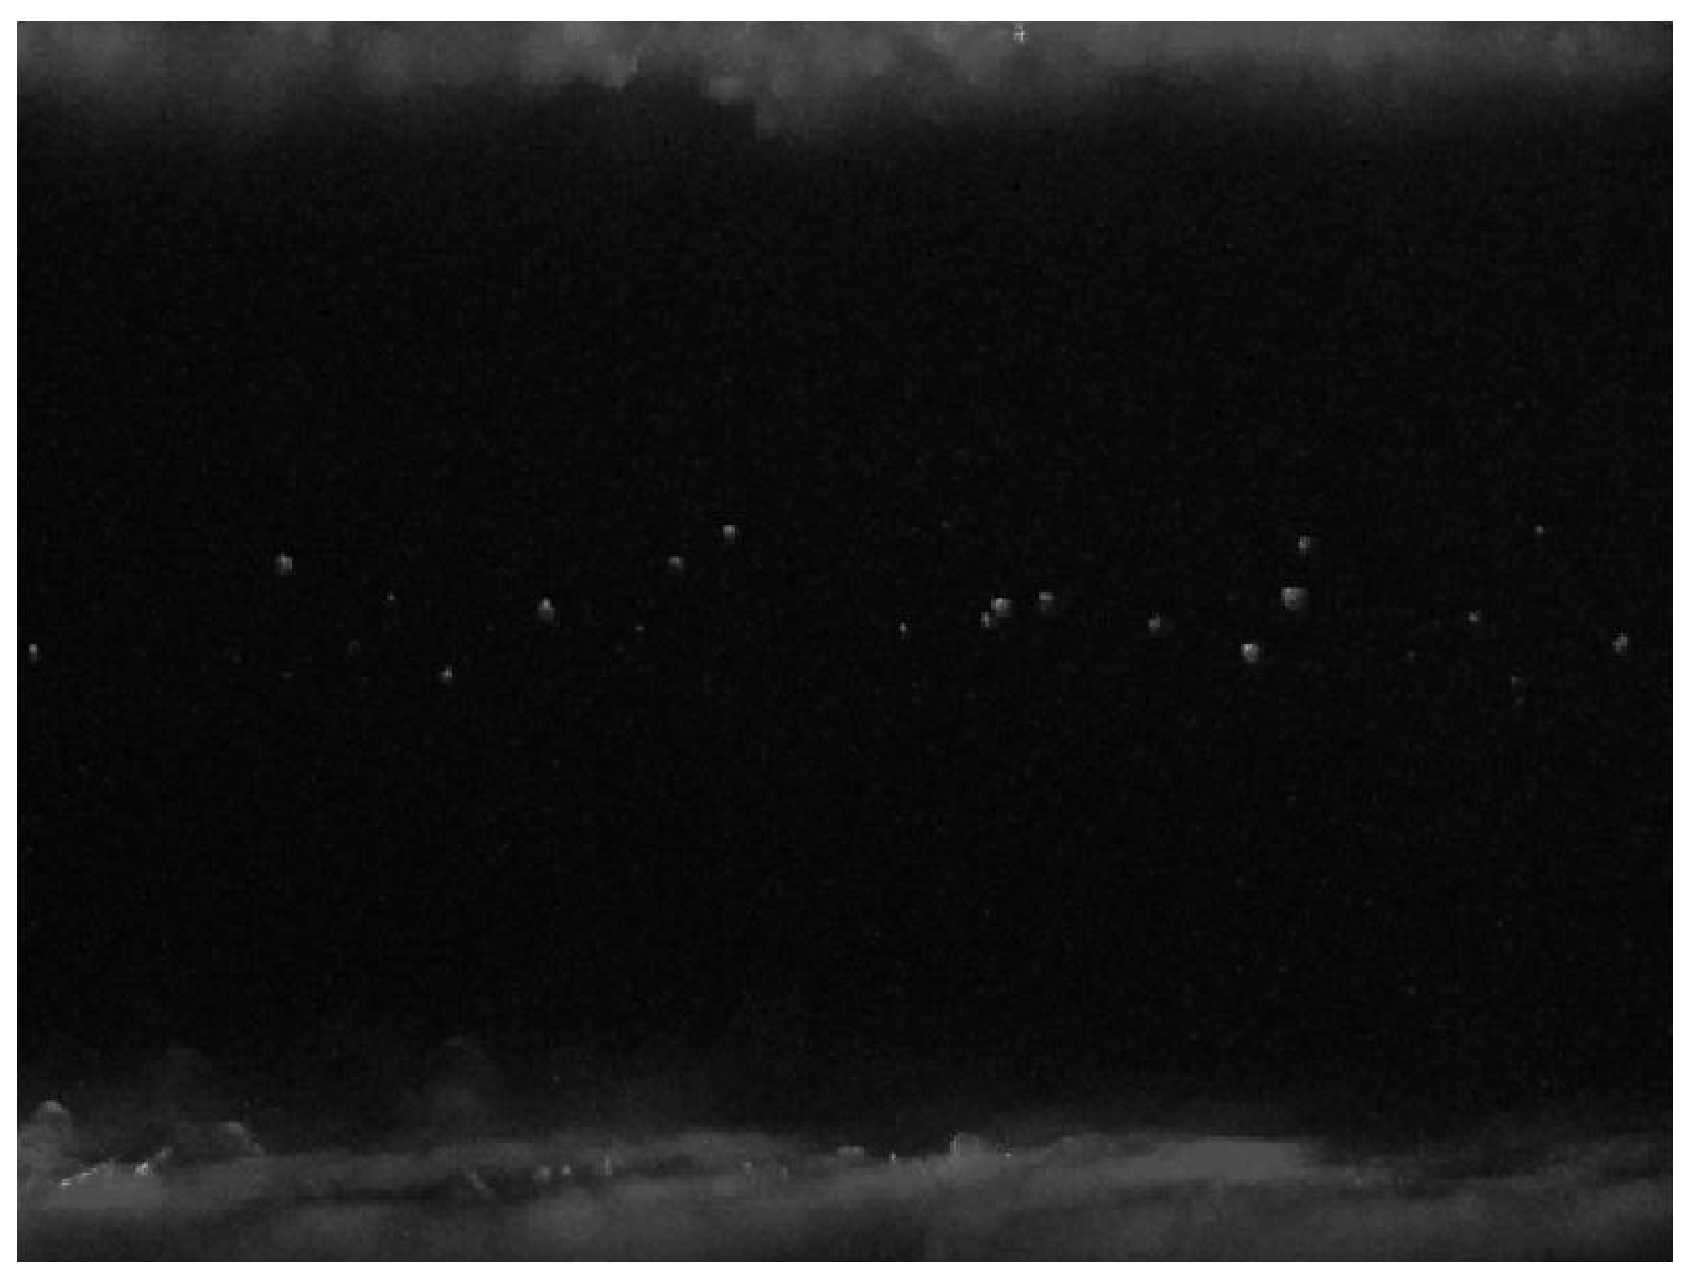
\includegraphics[scale=0.2]{epsGotas/c1.eps}} \qquad
\subfigure[]{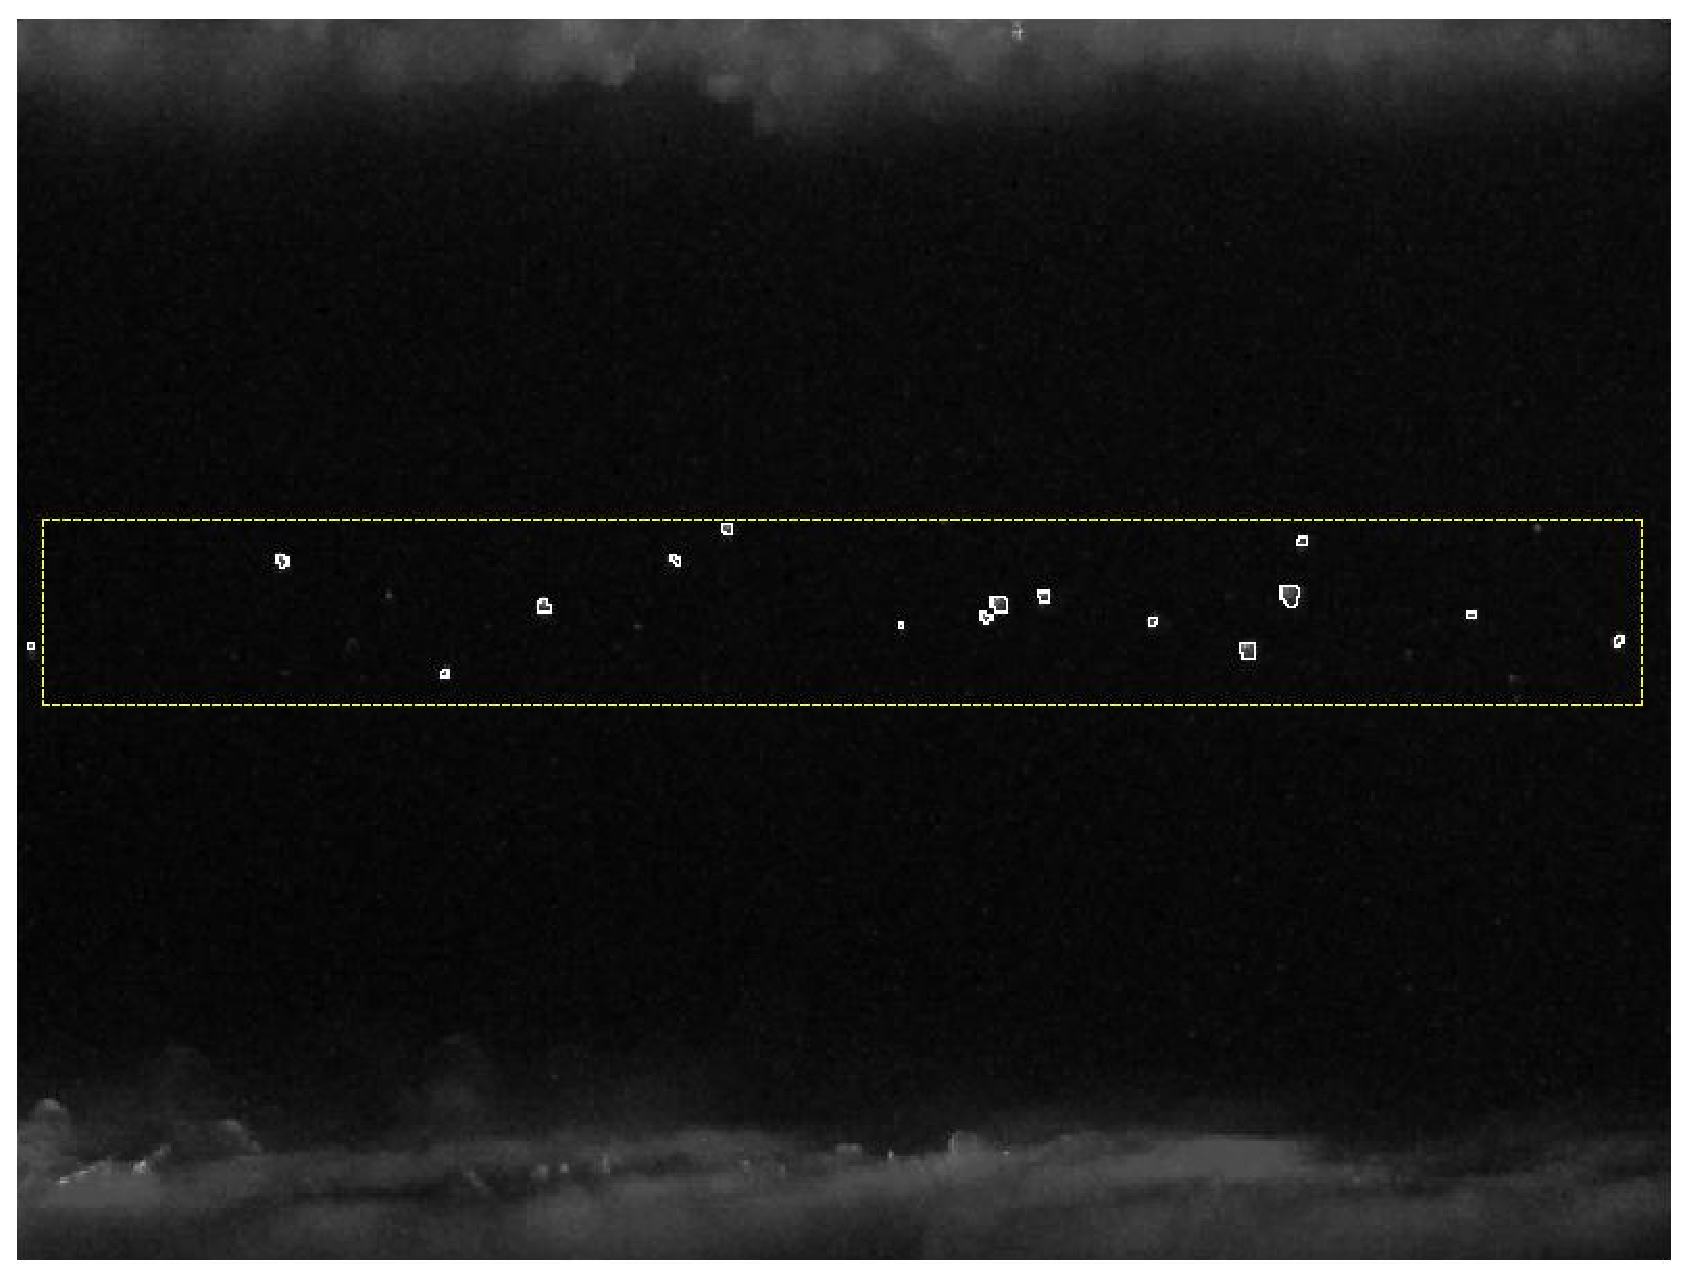
\includegraphics[scale=0.2]{epsGotas/c1Seg.eps}} \qquad
\centering \caption{15 gotas (528 gotas/cm$^3$).}
\label{c1}
\end{figure}

\begin{figure}[!htbp]%
\centering
\subfigure[]{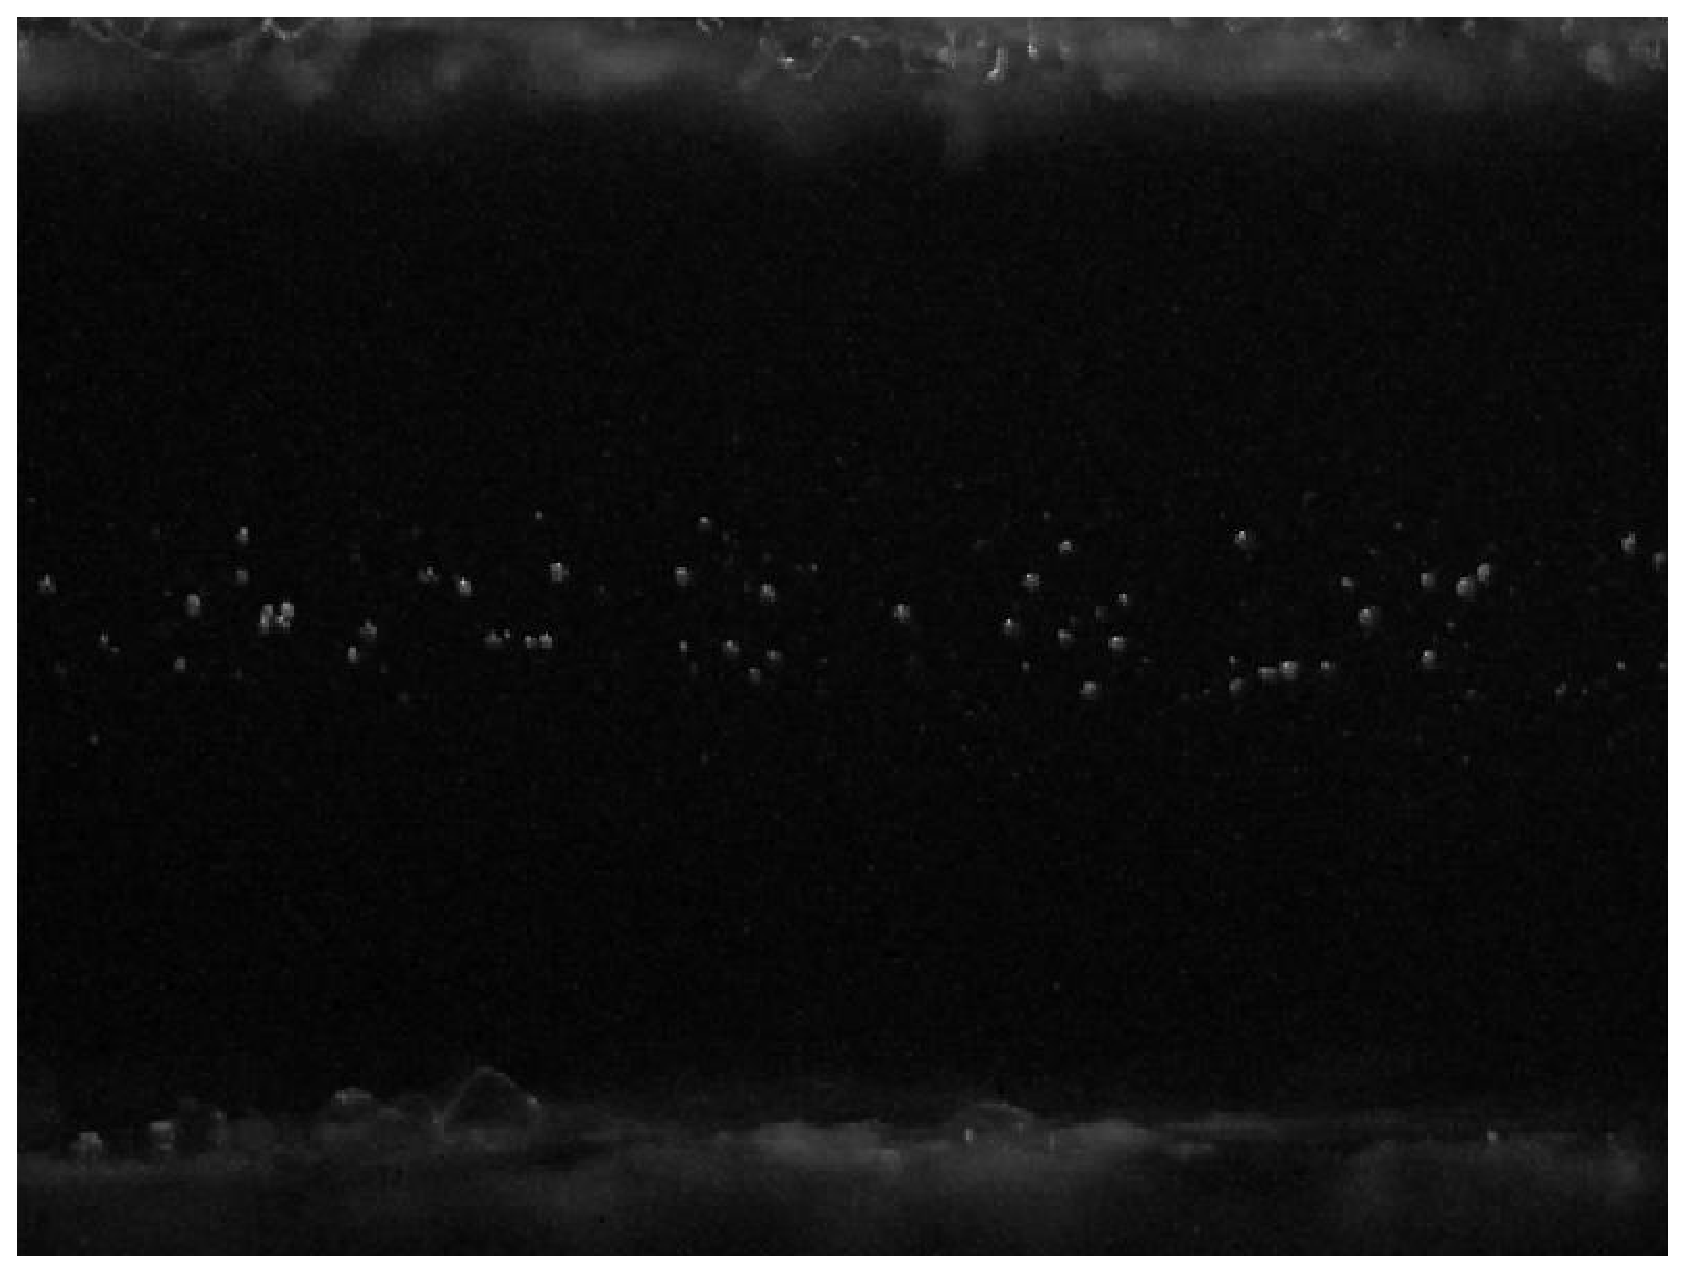
\includegraphics[scale=0.2]{epsGotas/c2.eps}} \qquad
\subfigure[]{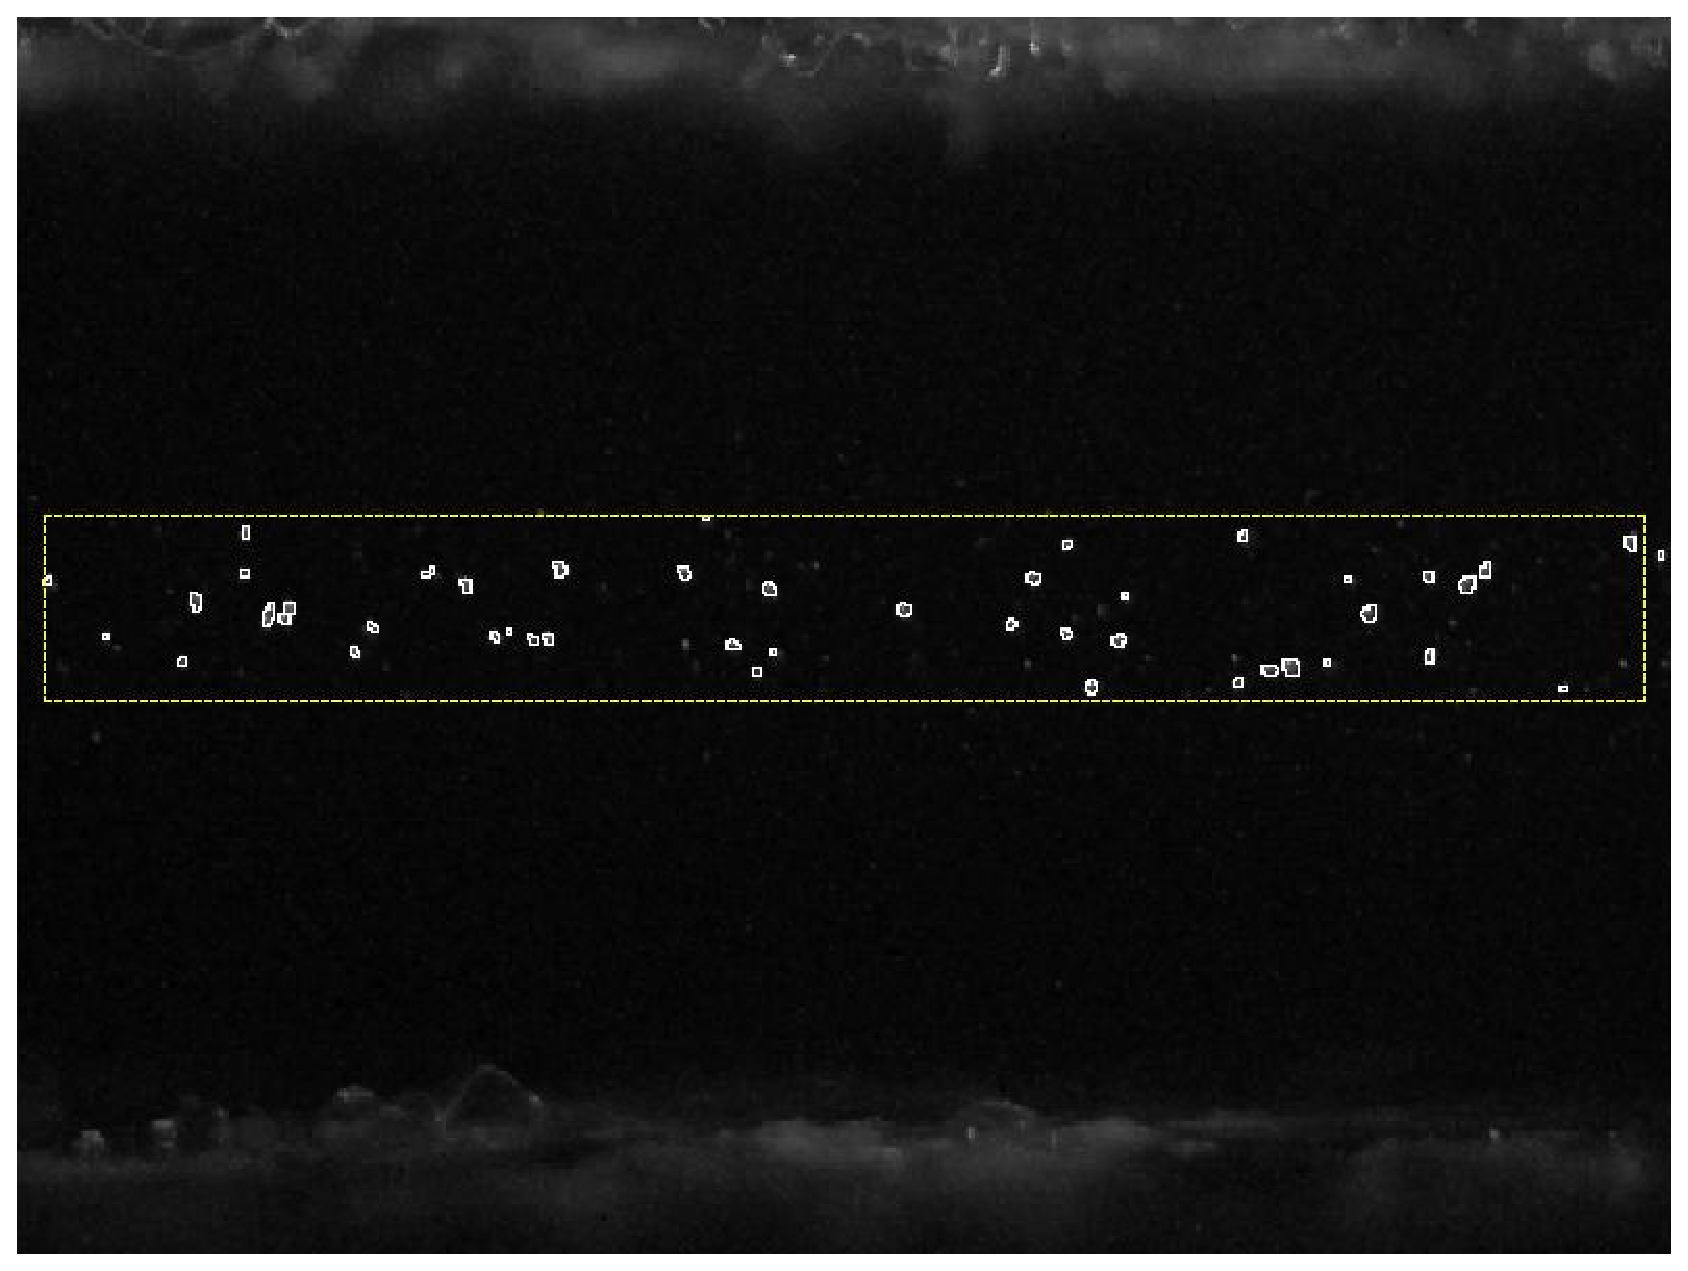
\includegraphics[scale=0.2]{epsGotas/c2Seg.eps}} \qquad
\centering \caption{48 gotas (1616 gotas/cm$^3$).}
\label{c2}
\end{figure}


\begin{figure}[!htbp]%
\centering
\subfigure[]{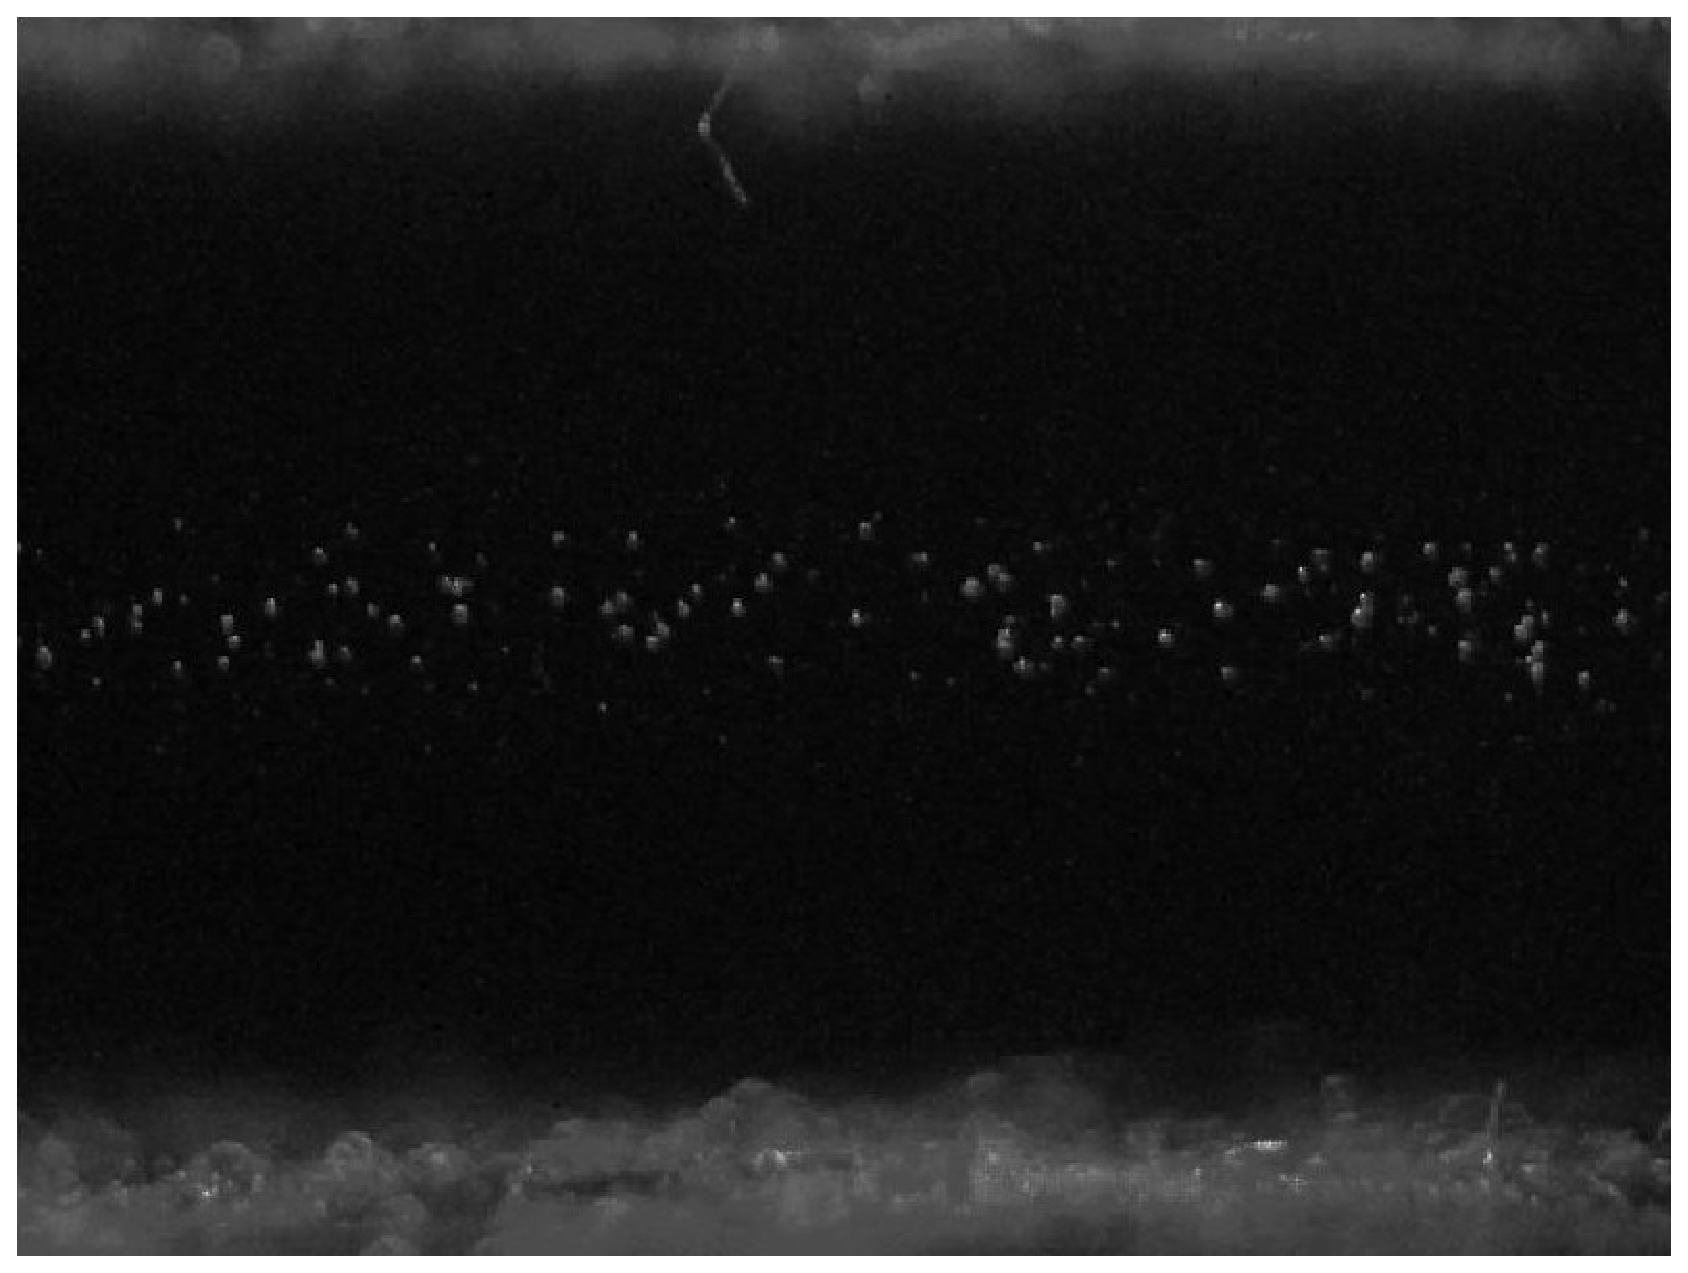
\includegraphics[scale=0.2]{epsGotas/c3.eps}} \qquad
\subfigure[]{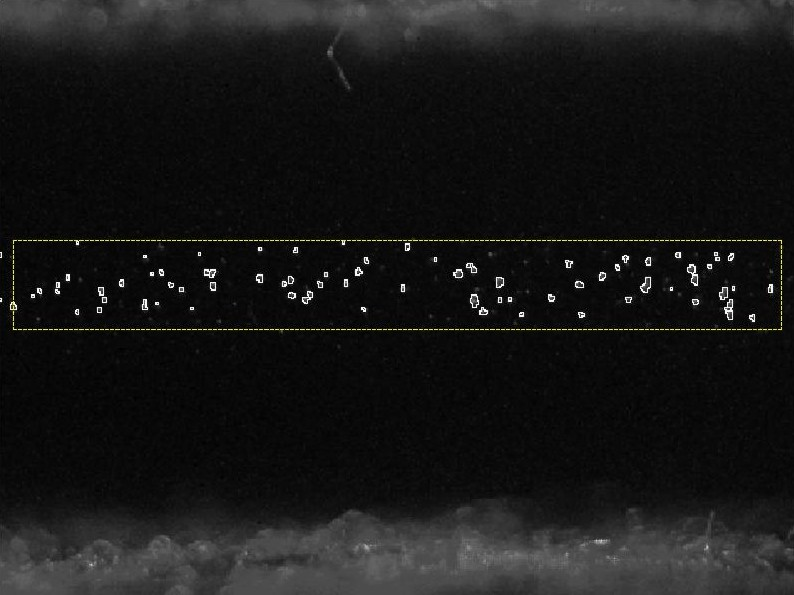
\includegraphics[scale=0.2]{epsGotas/c3Seg.eps}}
\centering \caption{83 gotas (2774 gotas/cm$^3$).}
\label{c3}
\end{figure}

\begin{figure}[!htbp]%
\centering
\subfigure[]{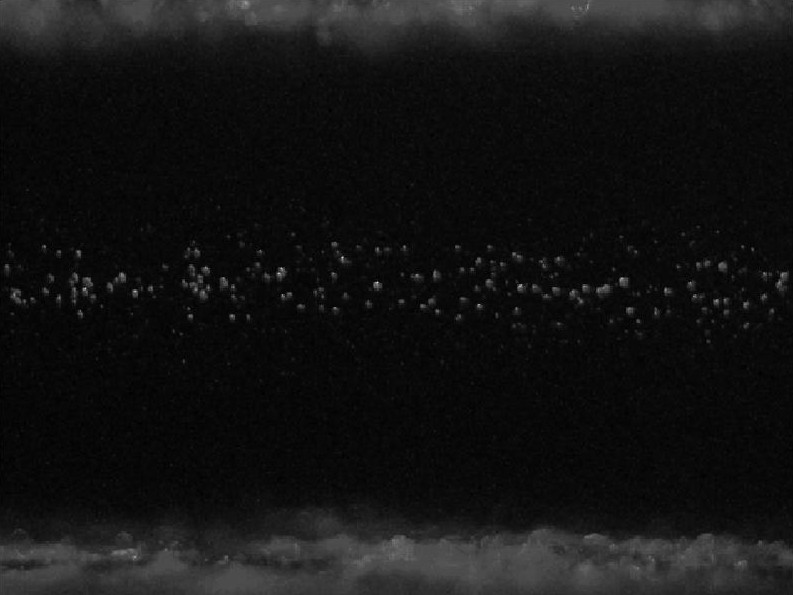
\includegraphics[scale=0.2]{epsGotas/c4.eps}} \qquad
\subfigure[]{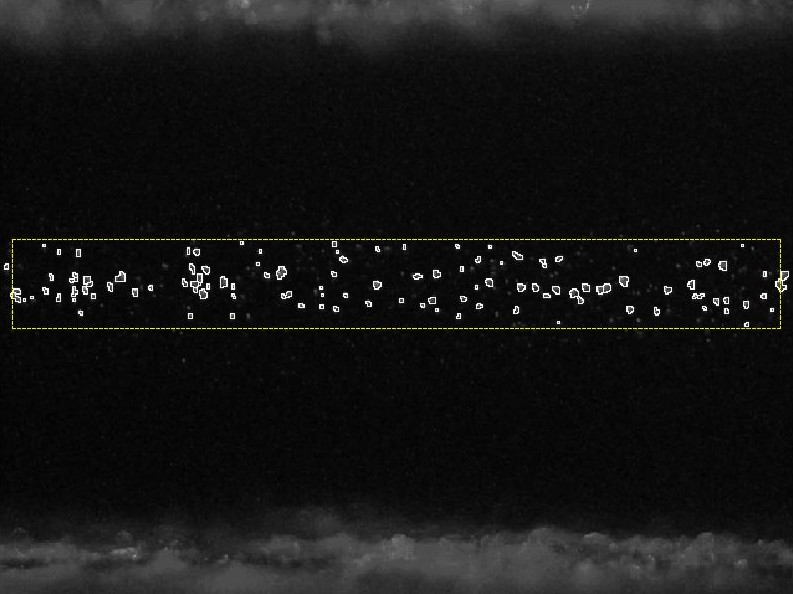
\includegraphics[scale=0.2]{epsGotas/c4Seg.eps}}
\centering \caption{124 gotas (4129 gotas/cm$^3$).}
\label{c4}
\end{figure}

\begin{figure}[!htbp]%
\centering
\subfigure[]{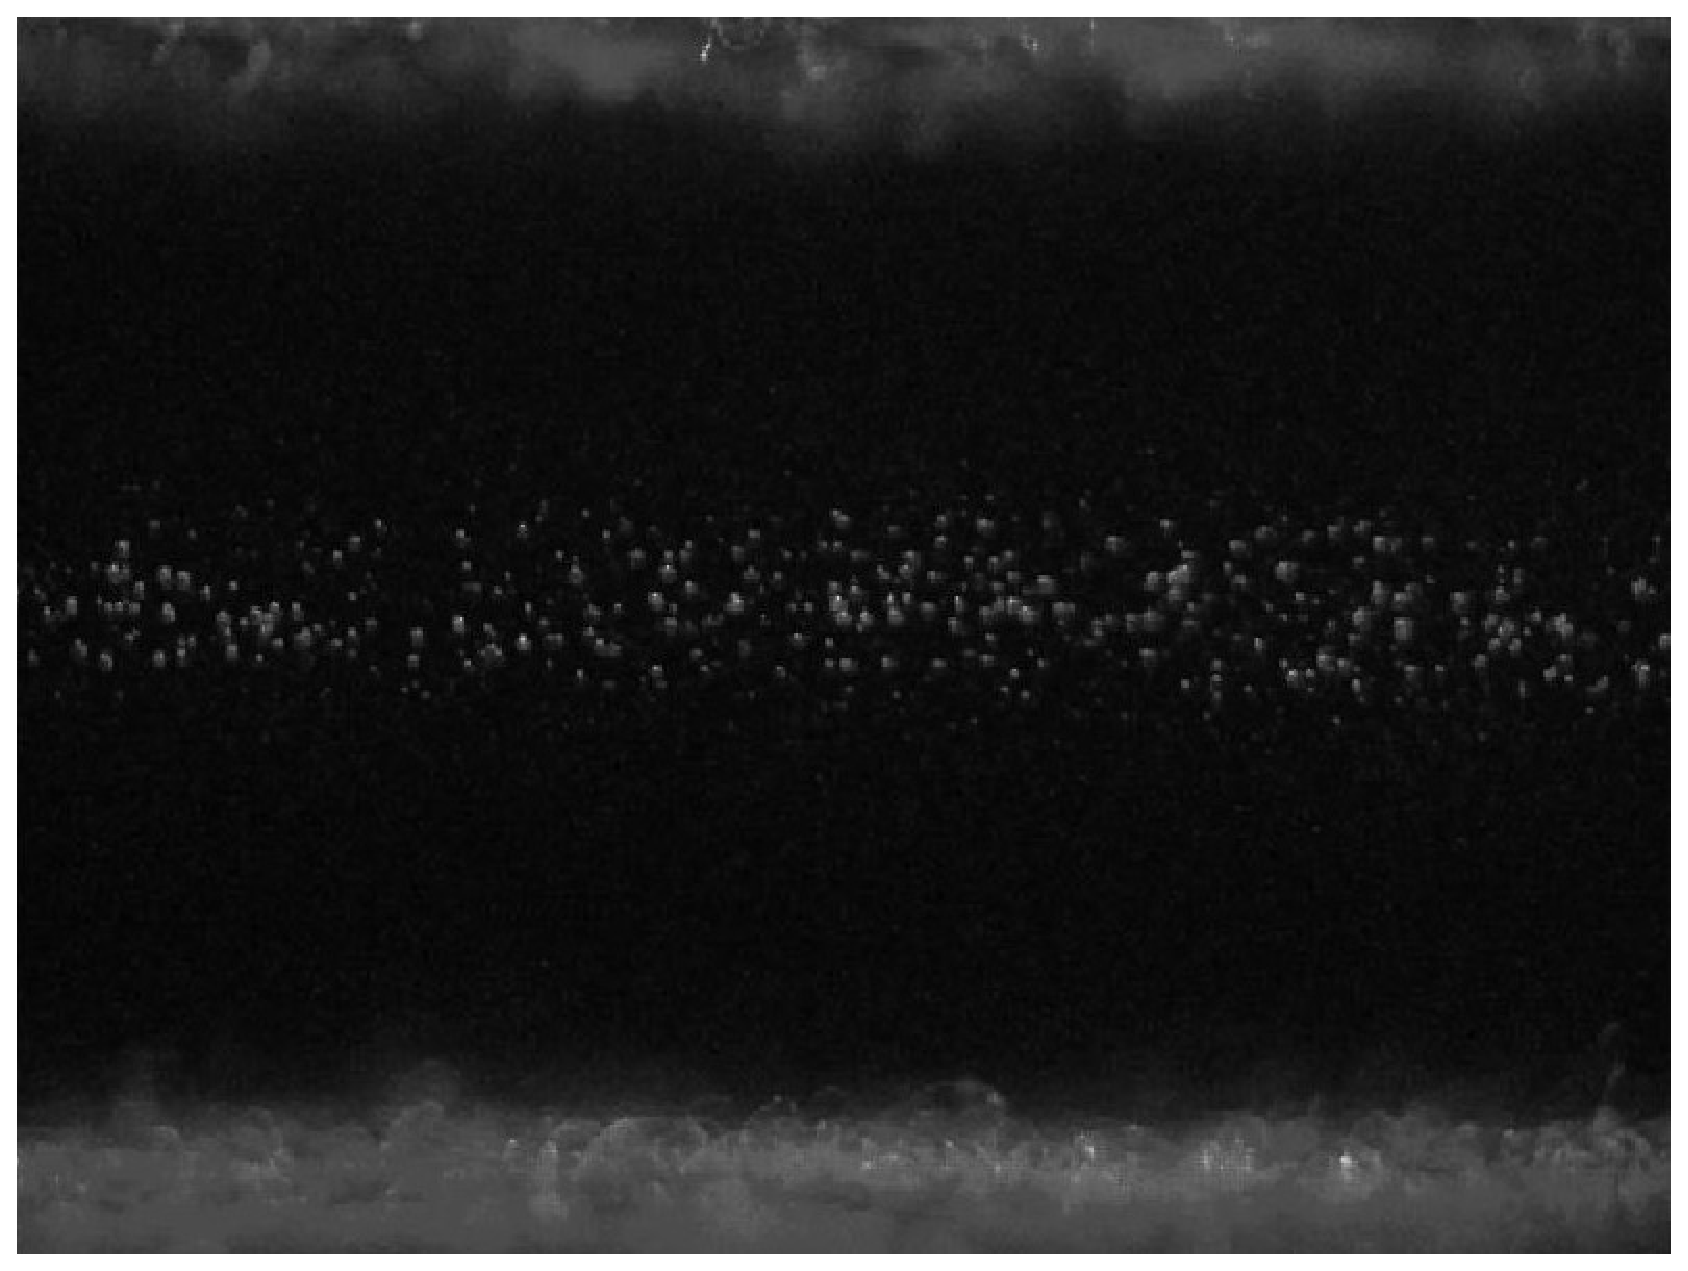
\includegraphics[scale=0.2]{epsGotas/c5.eps}} \qquad
\subfigure[]{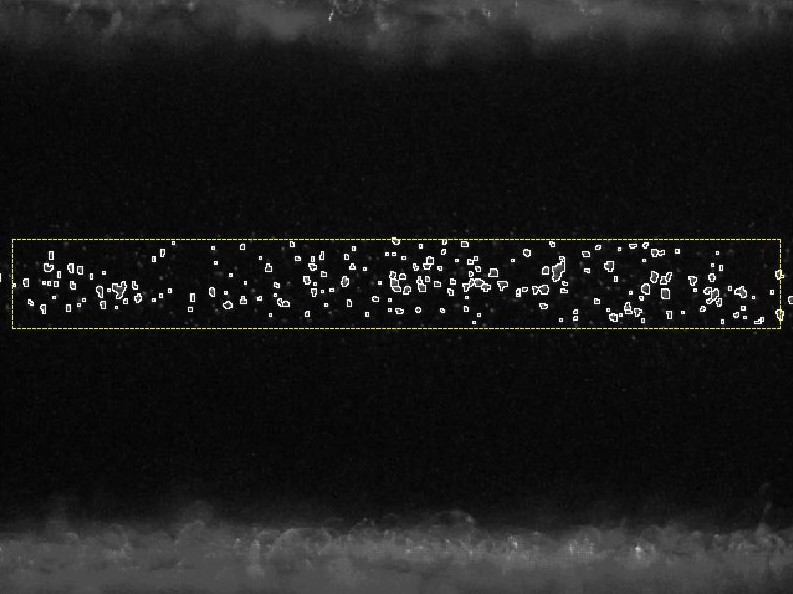
\includegraphics[scale=0.2]{epsGotas/c5Seg.eps}}
\centering \caption{191 gotas (6342 gotas/cm$^3$).}
\label{c5}
\end{figure}


Um exemplo da capacidade do sistema de vis\~{a}o computacional proposto em segmentar gotas sobrepostas \'{e} apresentado na Figura \ref{detseg}(a)  com destaque de uma regi\~{a}o da imagem onde aparecem tr\^{e}s gotas muito pr\'{o}ximas. Ampliando-se essa regi\~{a}o, observa-se que tr\^{e}s gotas est\~{a}o parcialmente sobrepostas. Essa \'{e} uma situa\c{c}\~{a}o comum em altas concentra\c{c}\~{o}es em que uma segmenta\c{c}\~{a}o simples por binariza\c{c}\~{a}o implicaria em uma subcontagem e, por conseguinte, uma medida da concentra\c{c}\~{a}o menor do que a realidade apresenta. Entretanto, mesmo nessa condi\c{c}\~{a}o de sobreposi\c{c}\~{a}o parcial, o sistema de vis\~{a}o computacional utilizado  \'{e} capaz de identificar e isolar estes objetos (gotas) como pode ser visto no detalhe a direita, na mesma Figura, que \'{e} o resultado da segmenta\c{c}\~{a}o dessa regi\~{a}o da imagem. Na Figura \ref{detseg}(b) \'{e} apresentado o resultado da segmenta\c{c}\~{a}o na forma matricial em que os \emph{pixels} associados ao fundo da imagem s\~{a}o representados pelo n\'{u}mero 1; o contorno dos objetos s\~{a}o representados pelo n\'{u}mero 0 e  aos objetos (gotas) s\~{a}o representados pelos demais n\'{u}meros.

Nas condi\c{c}\~{o}es apresentadas na Figura \ref{detseg}, a contagem por um operador se torna praticamente imposs\'{\i}vel, bem como utilizando-se a contagem por espalhamento de luz. Este resultado evidencia a superioridade do CCNC-SDCC proposto em rela\c{c}\~{a}o aos CCNCs existentes que subestimam a medi\c{c}\~{a}o em concentra\c{c}\~{o}es acima de 3000 gotas/cm$^3$ \cite{Rose} devido a sobreposi\c{c}\~{a}o de gotas.



\begin{figure}[!htbp]%
\centering
\subfigure[]{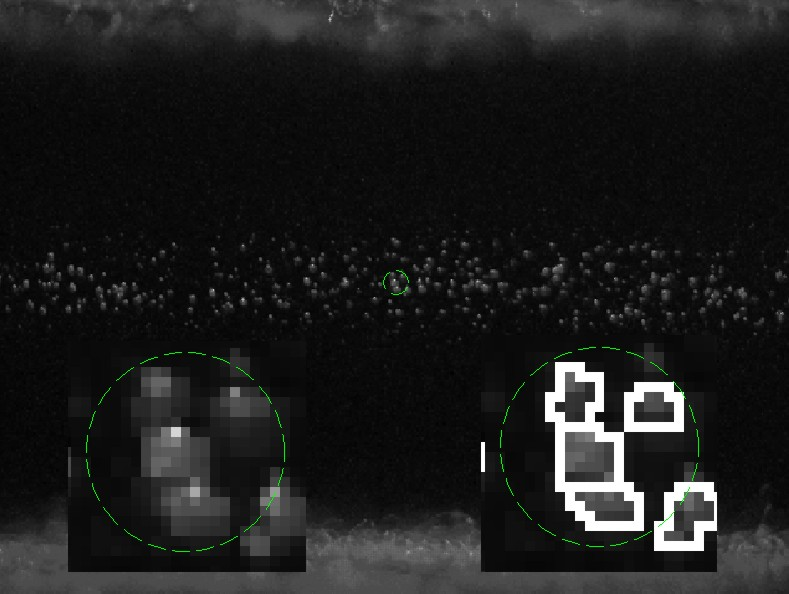
\includegraphics[scale=0.5]{epsGotas/gotaSegDetalhado.eps}} \\
\subfigure[]{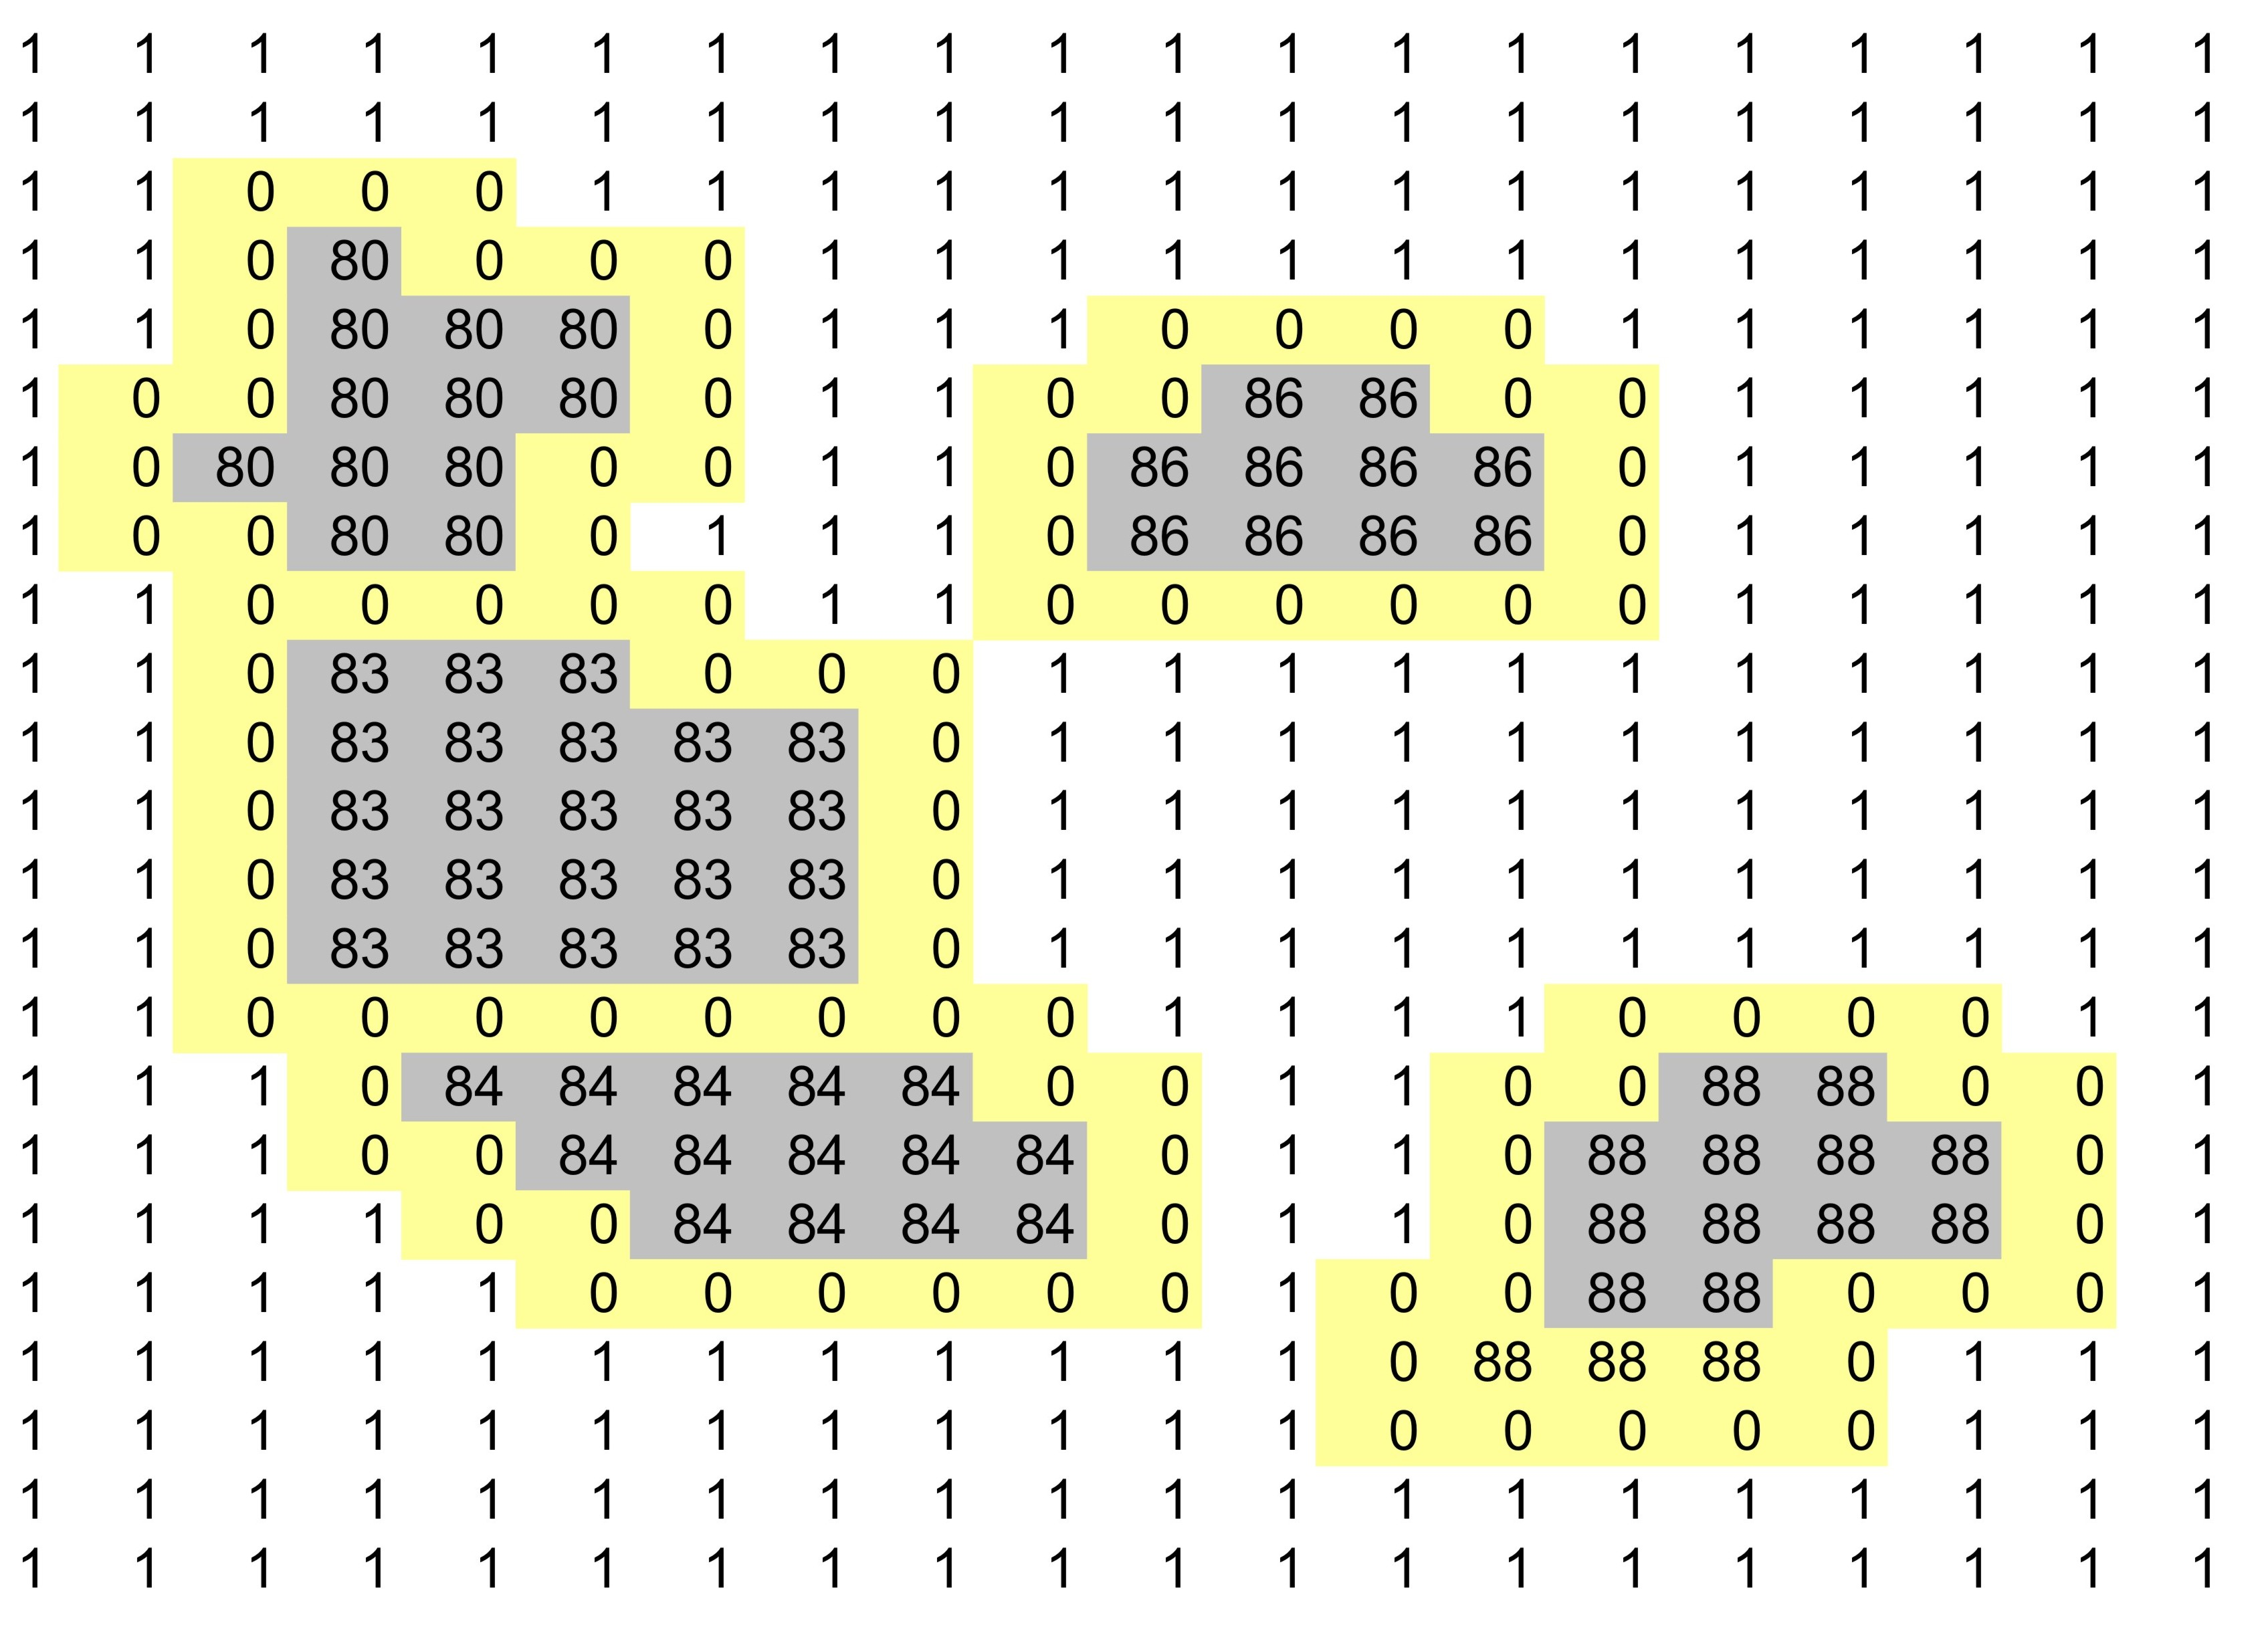
\includegraphics[scale=0.8]{epsGotas/TabelaGotas.eps}}
\centering \caption{resultado do CCNC-SDCC com gotas sobrepostas. (a) Imagem resultante do processo de segmenta\c{c}\~{a}o com expans\~{a}o de uma regi\~{a}o. (b) Representa\c{c}\~{a}o da regi\~{a}o expandida com a identifica\c{c}\~{a}o da gotas.}
\label{detseg}
\end{figure}




\section{Metodologia para avalia\c{c}\~{a}o de desempenho do CCNC-SDCC em bancada}

A metodologia para avalia\c{c}\~{a}o de desempenho do CCNC-SDCC em bancada consiste praticamente na mesma que foi utilizado por Frank et al. \cite{Frank}.  Isto \'{e}, foi realizada uma compara\c{c}\~{a}o entre um contador de part\'{\i}culas condens\'{a}veis CPC (\emph{Condensation Particle Counter} Modelo 3025) e o CCNC-SDCC. De uma forma resumida pode-se dizer que essa metodologia consiste em produzir uma concentra\c{c}\~{a}o de aeross\'{o}is capazes de, na sua totalidade, serem detectados pelo CCNC-SDCC e pelo CPC e comparar os resultados. Considerando-se que o CPC \'{e} um contador de part\'{\i}culas totais \'{e} importante que cada aerosol produzido seja exclusivamente formado por n\'{u}cleos higrosc\'{o}picos com um  di\^{a}metro m\'{\i}nimo de 100 nm, pois, nestas condi\c{c}\~{o}es, garante-se uma efici\^{e}ncia de detec\c{c}\~{a}o de 100\% por parte do CCNC-SDCC  \cite{HSU}. Nessas condi\c{c}\~{o}es, o que um instrumento detecta, o outro tamb\'{e}m deve detectar.

Para tal, foi utilizada no Laborat\'{o}rio de Qu\'{\i}mica da Part\'{\i}cula do Instituto Max Planck na Universidade de Mainz - Alemanha, uma bancada capaz de produzir aeross\'{o}is sob condi\c{c}\~{o}es controladas de concentra\c{c}\~{a}o, bem como de di\^{a}metro de part\'{\i}cula. Na Figura \ref{bga} s\~{a}o apresentados os diversos componentes da bancada: compressor, armadilha, atomizador, reservat\'{o}rio de sulfato de am\^{o}nia, secador, classificador eletrost\'{a}tico e o contador de part\'{\i}culas. Maiores detalhes dos equipamentos utilizados nessa bancada e seu funcionamento est\~{a}o no Anexo B.




\begin{figure}[htb]
\begin{center}
\includegraphics[scale=0.7]{eps/bga2.eps}\\
\end{center}
\caption{\label{bga}\hspace{-0.1em} bancada geradora de aeross\'{o}is.}
\end{figure}

\subsection{Aspectos pr\'{a}ticos do processo de compara\c{c}\~{a}o}
Considerando-se que este trabalho envolve fen\^{o}menos f\'{\i}sicos reais, algumas considera\c{c}\~{o}es do ponto de vista pr\'{a}tico, no que diz respeito ao ajuste de concentra\c{c}\~{a}o, sua varia\c{c}\~{a}o e seus transit\'{o}rios, s\~{a}o importantes de serem postas.


\subsubsection {Ajuste da concentra\c{c}\~{a}o de aeross\'{o}is}
O ajuste da concentra\c{c}\~{a}o de aeross\'{o}is \'{e} feito de forma emp\'{\i}rica. Isto \'{e}, dissolve-se o sulfato de am\^{o}nia em \'{a}gua destilada em uma propor\c{c}\~{a}o que corresponda a  uma dada concentra\c{c}\~{a}o que se deseja medir no CPC. Pequenas corre\c{c}\~{o}es podem ser realizadas, adicionando-se \'{a}gua destilada ou sulfato de am\^{o}nia para redu\c{c}\~{a}o ou aumento da concentra\c{c}\~{a}o, respectivamente. Outra forma de se obter pequenos ajustes \'{e} aumentando ou diminuindo a press\~{a}o de ar comprimido no sistema atrav\'{e}s de uma v\'{a}lvula.


Foram definidas tr\^{e}s faixas de valores de concentra\c{c}\~{o}es para realiza\c{c}\~{a}o dos experimentos de compara\c{c}\~{a}o:
\begin {itemize}
\item baixa ... < 1500 part\'{\i}culas $\cdot$ cm$^{-3}$,
\item m\'{e}dia.....  1500 - 3000 part\'{\i}culas $\cdot$ cm$^{-3}$ e
\item alta......> 3000 part\'{\i}culas $\cdot$ cm$^{-3}$.
\end{itemize}

\noindent Essas faixas de valores de concentra\c{c}\~{a}o de part\'{\i}culas s\~{a}o escolhidas pelo fato de representarem situa\c{c}\~{o}es normalmente encontradas na natureza \cite{Andreae}.




\subsubsection {Varia\c{c}\~{a}o da concentra\c{c}\~{a}o}
A concentra\c{c}\~{a}o medida pelo CPC varia ao logo do tempo como \'{e} mostrado na Figura \ref{concvar}. Essa varia\c{c}\~{a}o \'{e} uma consequ\^{e}ncia do processo de produ\c{c}\~{a}o de aeross\'{o}is, devida a uma remo\c{c}\~{a}o de \'{a}gua e de sulfato em propor\c{c}\~{o}es diferentes. Este fen\^{o}meno, tem forte implica\c{c}\~{a}o no procedimento de compara\c{c}\~{a}o. Isto porque as m\'{e}dias de medidas obtidas em um longo per\'{\i}odo de tempo variam, portanto n\~{a}o devem ser consideradas, mas apenas a compara\c{c}\~{a}o da medi\c{c}\~{a}o obtida pelo CCNC-SDCC e a medi\c{c}\~{a}o obtida pelo CPC em um curto per\'{\i}odo de tempo.

\begin{figure}[hbt]
\begin{center}
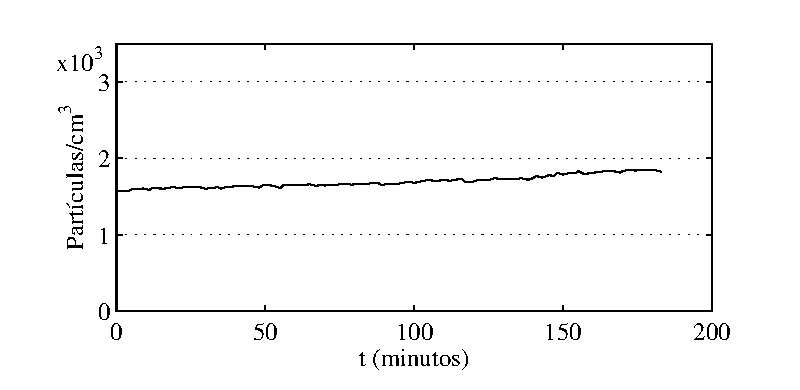
\includegraphics[scale=1.0]{GraficosMatlab/concvar.eps}\\
\end{center}
\caption{\label{concvar}\hspace{-0.1em} varia\c{c}\~{a}o da concentra\c{c}\~{a}o da bancada geradora de aeross\'{o}is.}
\end{figure}



\subsubsection {Transit\'{o}rios}
O CPC foi projetado para trabalhar com um fluxo cont\'{\i}nuo de aeross\'{o}is. O modelo TSI3025A, utilizado como refer\^{e}ncia neste trabalho, possui uma bomba que procura sempre manter o fluxo de 0,3 litros/min de aeross\'{o}is constante em seu sistema de medi\c{c}\~{a}o. Como o CCNC-SDCC deve ser posto em paralelo com o CPC, ao ser acionada a sua bomba para a realiza\c{c}\~{a}o da medida, este sofre uma altera\c{c}\~{a}o moment\^{a}nea de fluxo, produzindo-se as grandes varia\c{c}\~{o}es destacadas na Figura \ref{transiente}. Por essa raz\~{a}o, estes transit\'{o}rios devem ser descartados no processo de compara\c{c}\~{a}o.

\subsubsection{Procedimentos adotados para compara\c{c}\~{a}o}
Os efeitos da varia\c{c}\~{a}o da concentra\c{c}\~{a}o ao longo do tempo, bem como os efeitos transit\'{o}rios impostos ao CPC, devido ao princ\'{\i}pio operacional do CCNC-SDCC imp\~{o}em restri\c{c}\~{o}es nos dados de sa\'{\i}da do CPC usado como refer\^{e}ncia no processo de compara\c{c}\~{a}o. Considera-se como medida v\'{a}lida do CPC, para efeito de compara\c{c}\~{a}o, as 50 \'{u}ltimas medidas antes do acionamento da bomba do CCNC-SDCC. Na Figura \ref{transiente} s\~{a}o destacadas as regi\~{o}es consideradas e descartadas do sinal do CPC no processo de compara\c{c}\~{a}o.

%ucpc_59.xls arquivo de origem de gr\'{a}fico
\begin{figure}[hbt]
\begin{center}
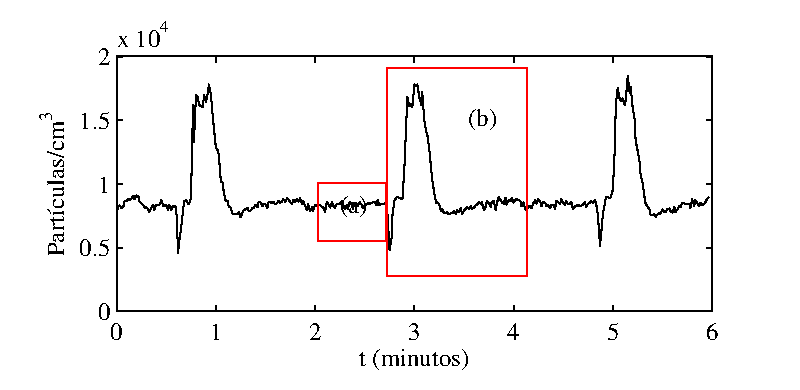
\includegraphics[scale=1.0]{GraficosMatlab/transiente.eps}\\
\end{center}
\caption{\label{transiente}\hspace{-0.1em} concentra\c{c}\~{a}o medida pelo CPC, destacando-se as regi\~{o}es usadas na medi\c{c}\~{a}o (a) e descartadas (b). }
\end{figure}


\section{Resultados da compara\c{c}\~{a}o entre o CCNC-SDCC e o CPC}
Os resultados s\~{a}o obtidos a partir da compara\c{c}\~{a}o entre o CCNC-SDCC e o CPC. Os medidores s\~{a}o montados de acordo com o que foi descrito no Cap\'{\i}tulo anterior, seguindo uma metodologia cl\'{a}ssica para este estudo  e que \'{e} apresentada por Frank et al. \cite{Frank}.

O processo de compara\c{c}\~{a}o apresentado na forma das Figuras  \ref{corr300} e \ref{corr100} indica uma forte correla\c{c}\~{a}o entre o CPC e o CCNC-SDCC. As correla\c{c}\~{o}es foram obtidas a partir de 297 medi\c{c}\~{o}es para o caso de part\'{\i}culas de 300 nm e de 55 medi\c{c}\~{o}es para ocaso de part\'{\i}culas de 100 nm.  A faixa de concentra\c{c}\~{a}o analisada \'{e} de 500 part\'{\i}culas/cm$^3$ at\'{e} 4500 part\'{\i}culas/cm$^3$. Essa \'{e} uma faixa bastante ampla que abrange desde situa\c{c}\~{o}es comumente encontradas nos processos de forma\c{c}\~{a}o de nuvens no oceano ou floresta (em situa\c{c}\~{o}es de baixa polui\c{c}\~{a}o), bem como em processo de forma\c{c}\~{a}o de nuvens produzidas por plumas de fuma\c{c}a oriundas de queima de florestas \cite{Andreae}.

\'{E} importante ressaltar que a \'{u}nica calibra\c{c}\~{a}o feita no CCNC-SDCC \'{e} aquela realizada na determina\c{c}\~{a}o do volume de amostragem. Isto \'{e}, n\~{a}o \'{e} feito nenhum ajuste nos dados obtidos. Este resultado demonstra claramente que o procedimento adotado para a medida do volume de amostragem, bem como as t\'{e}cnicas adotadas para contagem das gotas s\~{a}o adequados para essa aplica\c{c}\~{a}o. Dessa forma, este CCNC-SDCC dispensa equipamentos de refer\^{e}ncia para calibra\c{c}\~{a}o.

\begin{figure}[hbt]
\begin{center}
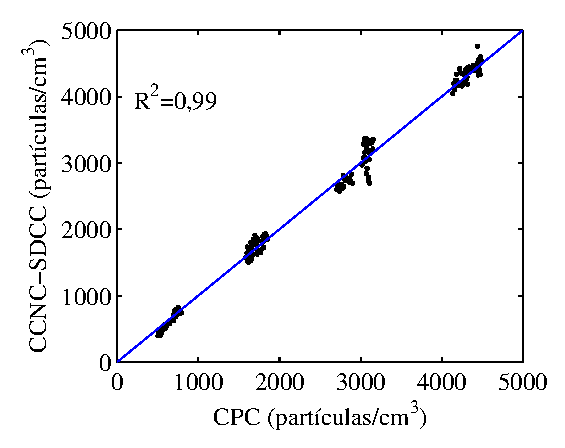
\includegraphics[scale=0.9]{GraficosMatlab/corr_300nm.eps}\\
\end{center}
\caption{\label{corr300}\hspace{-0.1em} correla\c{c}\~{a}o entre CPC e CCNC-SDCC utilizando aeross\'{o}is monodisperssivo de sulfato de am\^{o}nia com di\^{a}metro de 300 nm (297 pontos medidos). }
\end{figure}

\begin{figure}[hbt]
\begin{center}
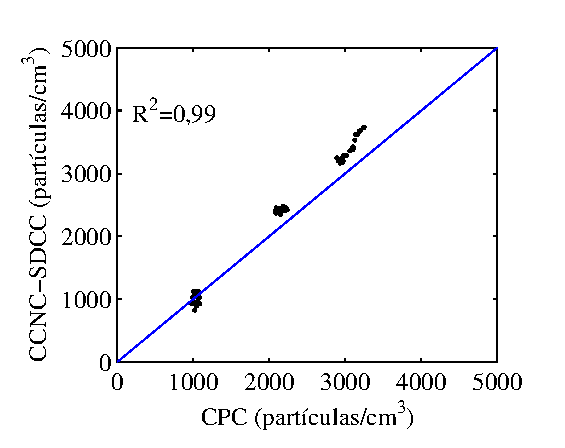
\includegraphics[scale=0.9]{GraficosMatlab/corr_100nm.eps}\\
\end{center}
\caption{\label{corr100}\hspace{-0.1em} correla\c{c}\~{a}o entre CPC e CCNC-SDCC utilizando aerossol monodisperssivo de sulfato de am\^{o}nia com di\^{a}metro de 100 nm (55 pontos medidos).}
\end{figure}

Outro aspecto importante que deve ser ressaltado \'{e} o que diz respeito \`{a} dispers\~{a}o dos dados. Na Figura \ref{dispersao} observa-se que o CCNC-SDCC possui um desvio padr\~{a}o relativo de 12\%, enquanto que o do CPC \'{e} de 7,4\% para o mesmo conjunto de dados.  Entretanto, na m\'{e}dia os valores s\~{a}o muito pr\'{o}ximos, conforme \'{e} demonstrado atrav\'{e}s das linhas de tend\^{e}ncias desenhadas na Figura \ref{dispersao}. O gr\'{a}fico apresentado na Figura \ref{dispersao} pode ser melhor compreendido na Figura \ref{hsterro} em que s\~{a}o apresentadas as distribui\c{c}\~{o}es dos erros do CPC (a) e do CCNC-SDCC (b) em rela\c{c}\~{a}o \`{a}s suas linhas de tend\^{e}ncias.


 A maior dispers\~{a}o no CCNC-SDCC em rela\c{c}\~{a}o ao CPC \'{e} esperada, pois, os aeross\'{o}is considerados s\~{a}o aqueles iluminados pela fonte de luz LASER que define o volume de amostragem.  Este volume \'{e} realmente  muito pequeno em rela\c{c}\~{a}o ao volume total da c\^{a}mara de nuvens, enquanto que no caso do CPC seu resultado \'{e} oriundo de uma m\'{e}dia, uma vez que seu sistema de medi\c{c}\~{a}o \'{e} de fluxo cont\'{\i}nuo. N\~{a}o se pode garantir, de forma pr\'{a}tica, uma distribui\c{c}\~{a}o espacial de gotas perfeitamente uniforme dentro da SDCC. Assim, cada medida considerada do CCNC-SDCC deve ser o resultado de uma m\'{e}dia aritm\'{e}tica em torno do ponto de interesse, de maneira semelhante ao que foi feito com os dados que originaram as Figuras \ref{corr300} e \ref{corr100}.

\begin{figure}[hbt]
\begin{center}
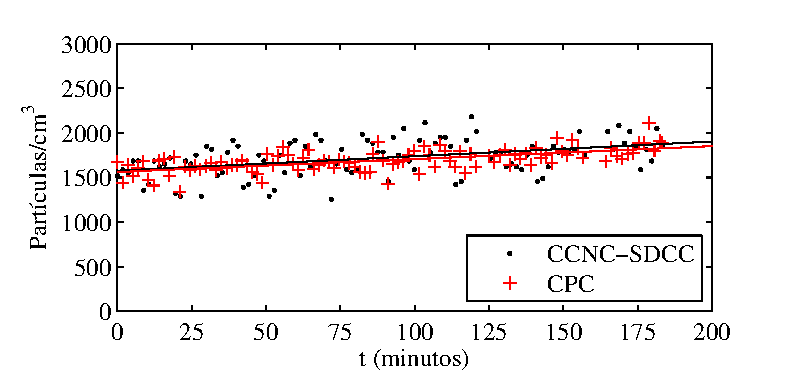
\includegraphics[scale=0.9]{GraficosMatlab/dispersao.eps}\\
\end{center}
\caption{\label{dispersao}\hspace{-0.1em} compara\c{c}\~{a}o da dispers\~{a}o dos dados entre CPC e o CCNC-SDCC  utilizando aeross\'{o}is monodisperssivo de sulfato de am\^{o}nia com di\^{a}metro de 100 nm.}
\end{figure}



\begin{figure}[!htbp]%
\centering
\subfigure[]{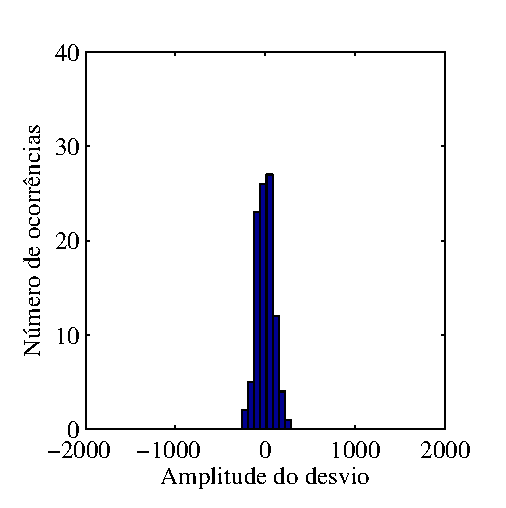
\includegraphics[scale=0.8]{GraficosMatlab/hstcpc.eps}} \qquad
\subfigure[]{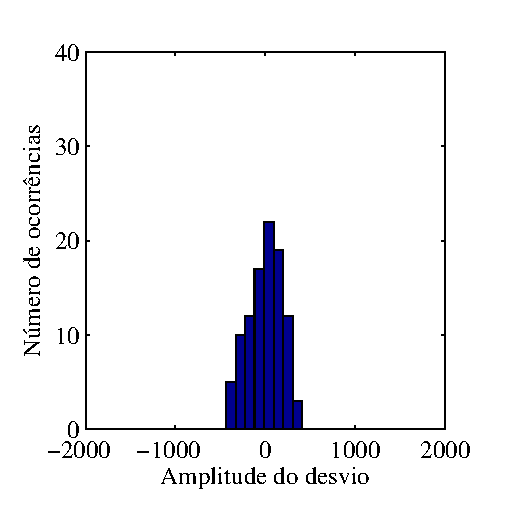
\includegraphics[scale=0.8]{GraficosMatlab/hstccnc.eps}} \qquad
\centering \caption{ dispress\~{a}o dos dados do CPC (a) e do CCNC (b) em rela\c{c}\~{a}o \`{a}s suas linhas de tend\^{e}ncia.}
\label{hsterro}
\end{figure}



%\begin{figure}[hbt]
%\begin{center}
%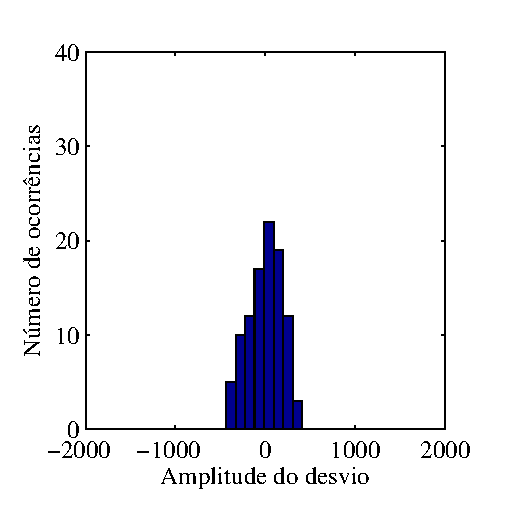
\includegraphics[scale=1.0]{GraficosMatlab/hstccnc.eps}\\
%\end{center}
%\caption{\label{hstccnc}\hspace{-0.1em} dispress\~{a}o dos dados do CCNC-SDCC em rela\c{c}\~{a}o a linha de tend\^{e}ncia. }
%\end{figure}


%\begin{figure}[hbt]
%\begin{center}
%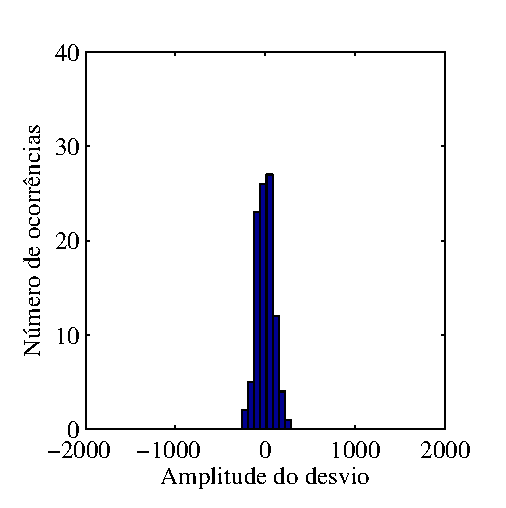
\includegraphics[scale=1.0]{GraficosMatlab/hstcpc.eps}\\
%\end{center}
%\caption{\label{hstcpc}\hspace{-0.1em} dispress\~{a}o dos dados do CPC em rela\c{c}\~{a}o a linha de tend\^{e}ncia. }
%\end{figure}



\section {Aspectos mec\^{a}nicos e el\'{e}tricos}
O CCNC-SDCC foi desenvolvido para substituir um outro CCNC, mais antigo, que atualmente \'{e} utilizado no Avi\~{a}o Laborat\'{o}rio para Pesquisas Atmosf\'{e}ricas - ALPA, o CCNC-WYO. Descrito no Cap\'{\i}tulo 2, o CCNC-WYO faz parte de um conjunto de equipamentos instalados no Avi\~{a}o Laborat\'{o}rio para Pesquisas Atmosf\'{e}ricas (ALPA) cuja finalidade \'{e} realizar as medidas de par\^{a}metros microf\'{\i}sicos das nuvens \textit{in situ} (temperatura ambiente, temperatura de ponto de orvalho, press\~{a}o atmosf\'{e}rica, quantidade de \'{a}gua l\'{\i}quida, espectro de gotas de nuvens e de chuva, concentra\c{c}\~{a}o de n\'{u}cleos de condensa\c{c}\~{a}o de nuvens dentre outros par\^{a}metros). O ALPA, uma aeronave modelo Bandeirante EMB110-P1, foi modificada tanto estruturalmente quanto eletricamente para receber este conjunto de equipamentos.

Nesse conjunto de equipamentos encontra-se o CCNC-WYO, que ocupa o maior espa\c{c}o e possui maiores peso e consumo de energia. Estes tr\^{e}s par\^{a}metros (peso, espa\c{c}o e consumo de energia) s\~{a}o restritivos em medi\c{c}\~{o}es aerotransportadas, pois, os recursos de espa\c{c}o e energia dentro da aeronave s\~{a}o limitados e o posicionamento do equipamento na aeronave em fun\c{c}\~{a}o do seu peso tamb\'{e}m imp\~{o}e restri\c{c}\~{o}es. Assim sendo, caso seja necess\'{a}rio incluir algum equipamento extra, situa\c{c}\~{a}o bastante comum, outro deve ser desligado e, \`{a}s vezes ser removido da aeronave por raz\~{o}es de seguran\c{c}a. Nesse contexto, o CCNC-SDCC apresenta significativa vantagem em rela\c{c}\~{a}o CCNC-WYO, pois, apresenta uma importante redu\c{c}\~{a}o de tais par\^{a}metros conforme mostra a Tabela \ref{alpaequip} possibilitando a instala\c{c}\~{a}o de outros equipamentos.



\begin{table}[!htbp]
\centering \caption{\label{alpaequip} compara\c{c}\~{a}o entre CCNC-SDCC e o CCNC-WYO.}
\begin{tabular}{ c | c c}
  \hline
  Par\^{a}metro & CCNC-SDCC & CCNC-WYO\\
  \hline
  Volume & 29,2 l & 40,0 l\\
  Peso & 5,0 kg & 37,0 kg\\
  Corrente m\'{e}dia & 0,35 A & 1,0 A\\
  Corrente de pico & 1,5 A & 3,0 A \\
  \hline
\end{tabular}\\
\end{table}

Na constru\c{c}\~{a}o do CCNC-SDCC foram utilizados componentes facilmente encontrados no mercado nacional. Apenas duas pe\c{c}as foram feitas sob encomenda: a c\^{a}mara de nuvens e a placa de circuito impresso da unidade de controle.

O prot\'{o}tipo do CCNC-SDCC foi montado em uma caixa padr\~{a}o de alum\'{\i}nio do tipo 19" X 3U. Alguns componentes ficaram externos \`{a} caixa como, por exemplo, o LASER, sua fonte de alimenta\c{c}\~{a}o, bem como parte da SDCC. Dessa forma, as dimens\~{o}es do CCNC-SDCC s\~{a}o as seguintes: 48,26cm de frente, 22,0cm de altura e 27,5cm de profundidade. Na Figura \ref{CCNC-SDCC} \'{e} apresentado o prot\'{o}tipo.

\begin{figure}[hbt]
\begin{center}
\includegraphics[scale=1.0]{eps/ccnclaptop.eps}\\
\end{center}
\caption{\label{CCNC-SDCC}\hspace{-0.1em} prot\'{o}tipo do CCNC-SDCC.}
\end{figure}

Nas Figuras \ref{CCNCxCCNC2} e \ref{ccncxccnc3} s\~{a}o apresentadas vistas frontais e superior, evidenciando uma boa percep\c{c}\~{a}o do ganho de espa\c{c}o obtido pelo CCNC-SDCC.


\begin{figure}[hbt]
\begin{center}
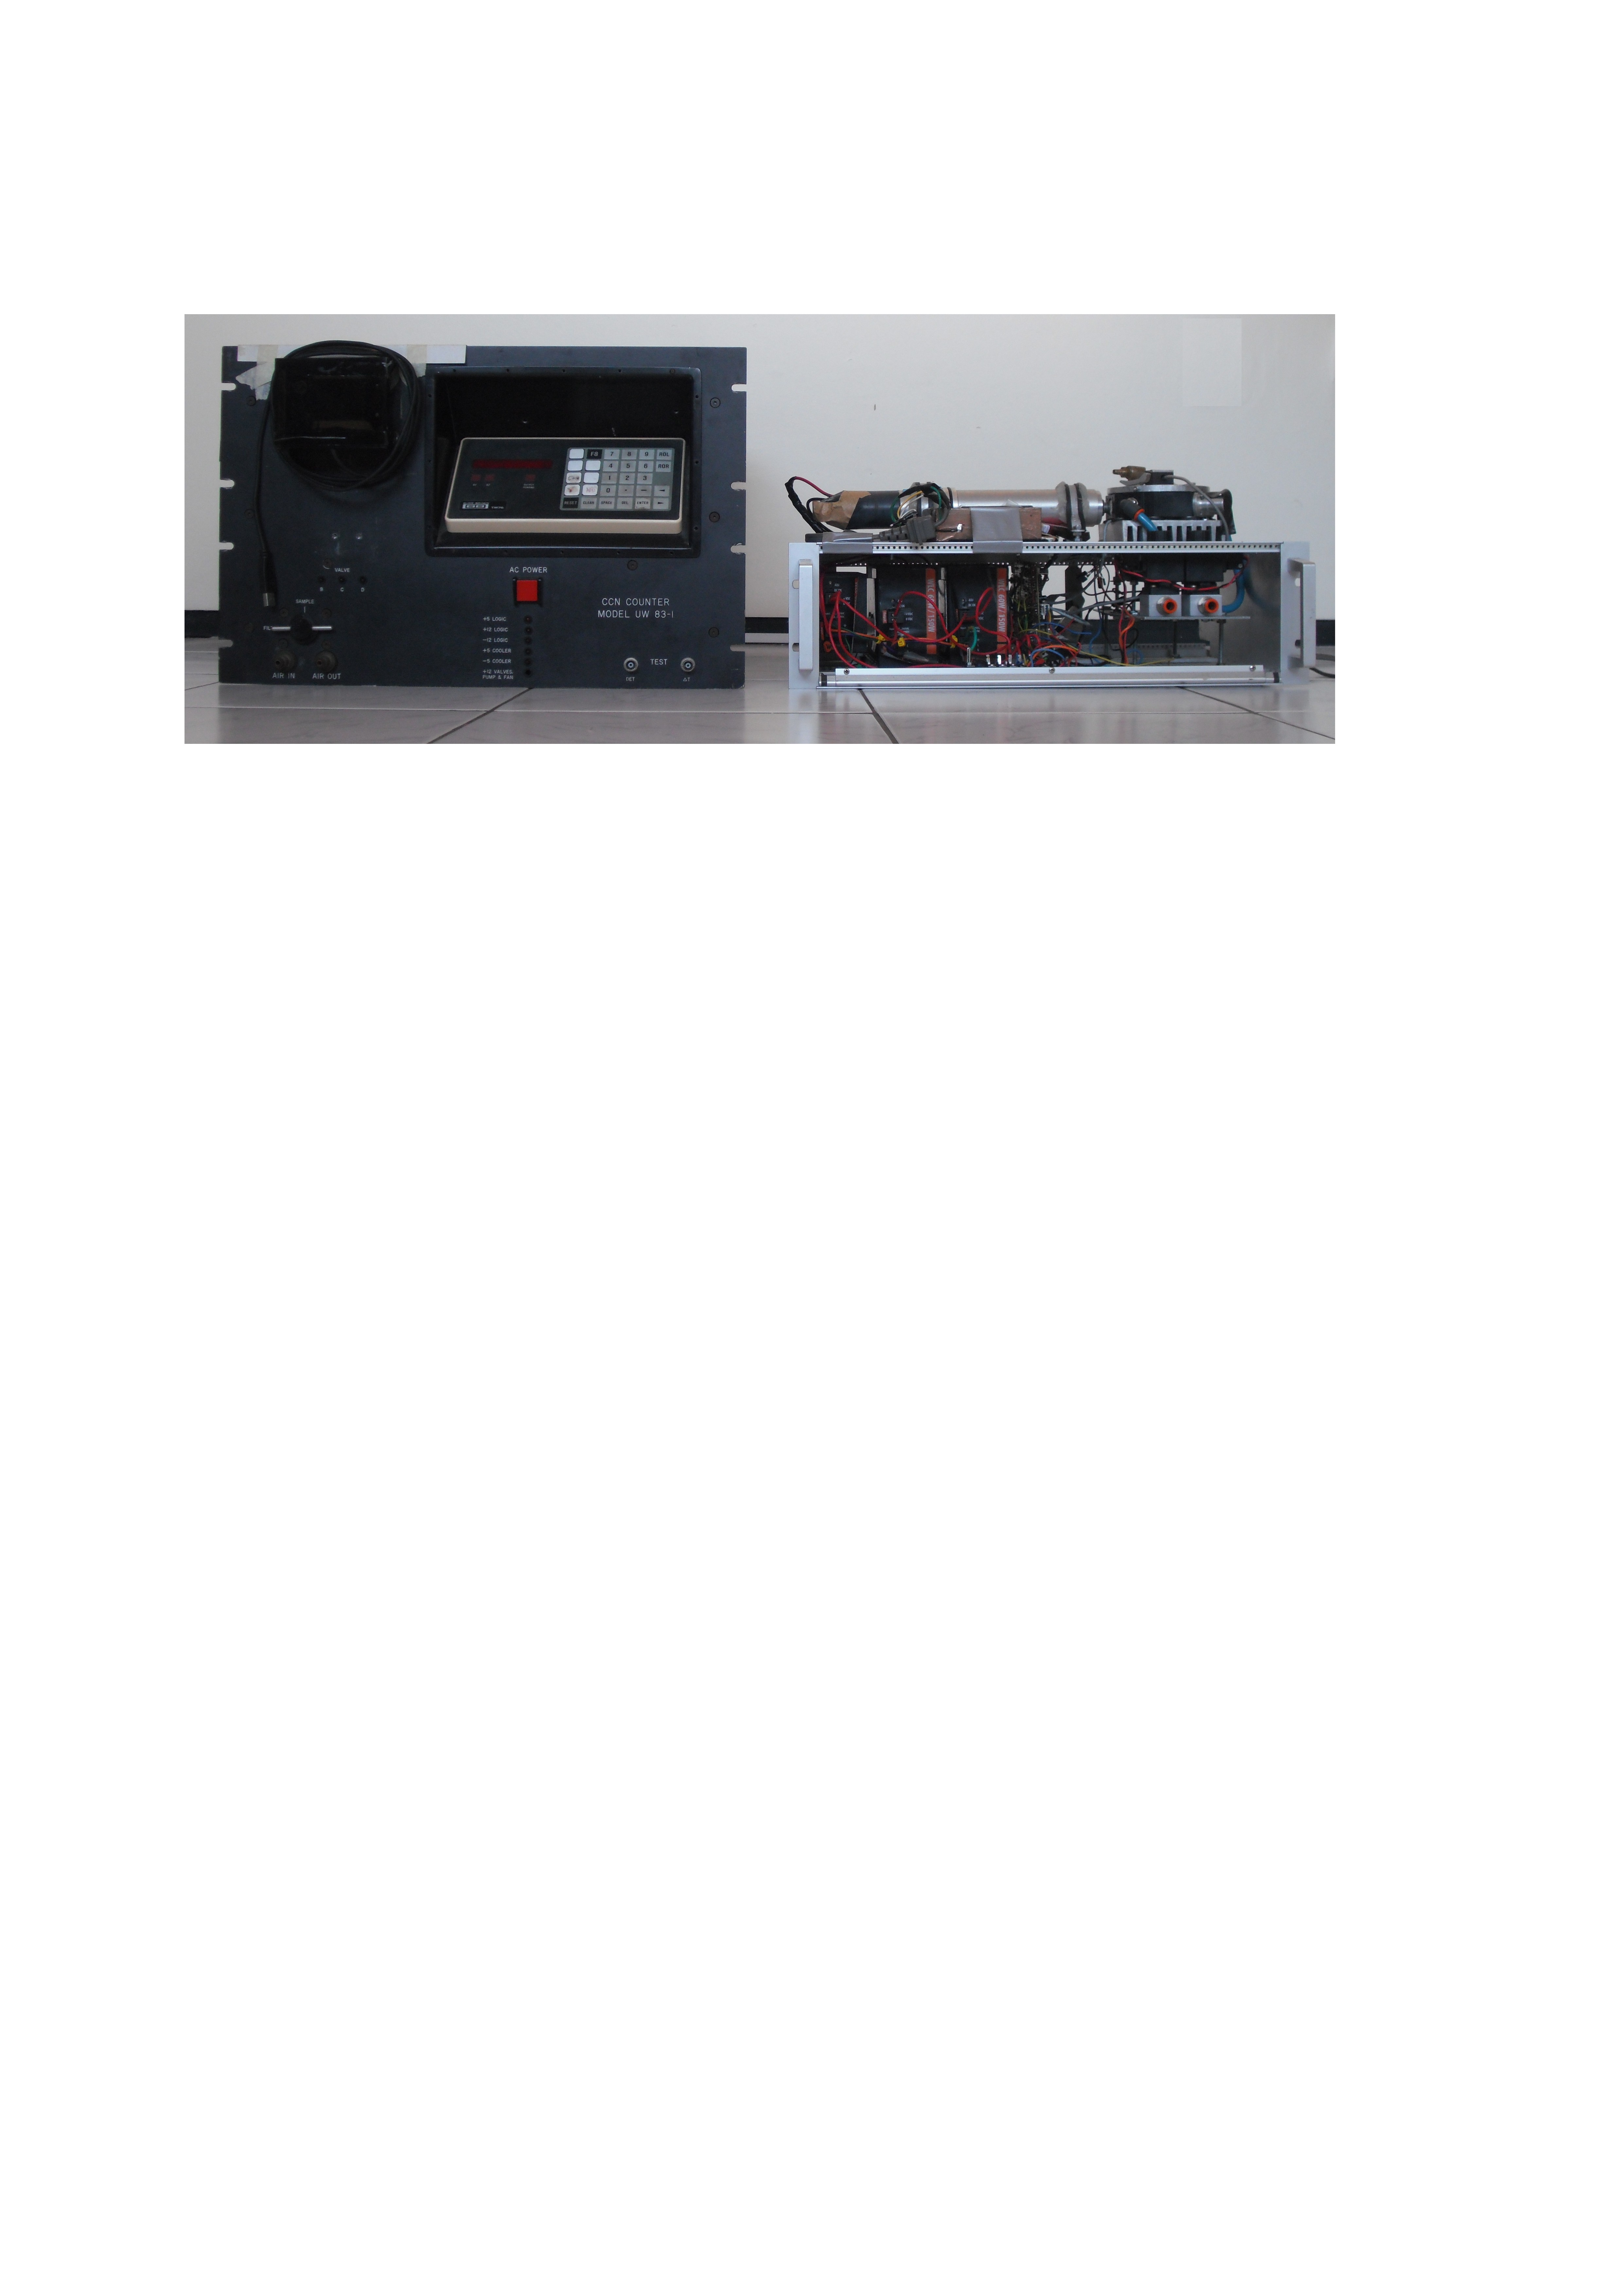
\includegraphics[scale=1.0]{eps/CCNCxCCNC2.eps}\\
\end{center}
\caption{\label{CCNCxCCNC2}\hspace{-0.1em} vista frontal dos dois CCNCs.}
\end{figure}


\begin{figure}[hbt]
\begin{center}
\includegraphics[scale=1.0]{eps/ccncxccnc3.eps}\\
\end{center}
\caption{\label{ccncxccnc3}\hspace{-0.1em} vista superior dos dois CCNCs.}
\end{figure}

